\documentclass[12pt, titlepage]{article}
\usepackage{placeins}
\usepackage{booktabs}
\usepackage{tabularx}
\usepackage{hyperref}
\usepackage{multirow}
\usepackage{graphicx}
\usepackage{caption}
\usepackage{subcaption}
\usepackage[normalem]{ulem}
\usepackage{xcolor}
\hypersetup{
    colorlinks,
    citecolor=black,
    filecolor=black,
    linkcolor=red,
    urlcolor=blue
}
\usepackage[round]{natbib}

\title{SE 3XA3: Test Plan\\BlockBuilder}

\author{Team 28, OAC
		\\ Andrew Lucentini, lucenta
		\\ Owen McNeil, mcneilo
		\\ Christopher DiBussolo, dibussoc
}

\date{\today}

%\input{../Comments}

\begin{document}

\maketitle

\pagenumbering{roman}
\tableofcontents
\listoftables
\listoffigures

\begin{table}[bp]
\caption{\bf Revision History}
\begin{tabularx}{\textwidth}{p{3cm}p{2cm}X}
\toprule {\bf Date} & {\bf Version} & {\bf Notes}\\
\midrule
October 26, 2018 & 1.0 & Initial push of Test Plan Doc.\\
\midrule
\textcolor{red}{December 1, 2018} & \textcolor{red}{2.0} & \textcolor{red}{Begin to make changes for Rev 1}\\
\midrule
\textcolor{red}{December 5, 2018} & \textcolor{red}{2.1} & \textcolor{red}{Final Rev1 changes pushed to repo}\\
\bottomrule
\end{tabularx}
\end{table}

\newpage

\pagenumbering{arabic}

This document elaborates on the testing methods that will be implemented during the development process of BlockBuilder.

\section{General Information}

\subsection{Purpose}

The purpose of testing this project is to ensure that all requirements are properly implemented in the software.      

\subsection{Scope}
This test plan will test the functional and non-functional requirements for BlockBuilder as well as provide a plan for individual testing of each function to ensure the software will work correctly and consistently.

\subsection{Acronyms, Abbreviations, and Symbols}
	
\begin{table}[hbp]
\caption{\textbf{Table of Abbreviations}} \label{Table}

\begin{tabularx}{\textwidth}{p{3cm}X}
\toprule
\textbf{Abbreviation} & \textbf{Definition} \\
\midrule
PoC & Proof of \sout{Conncept} \textcolor{red}{Concept}\\
POV & Point of view\\
GUI & Graphical User Interface\\
\bottomrule
\end{tabularx}

\end{table}

\begin{table}[!htbp]
\caption{\textbf{Table of Definitions}} \label{Table}

\begin{tabularx}{\textwidth}{p{3cm}X}
\toprule
\textbf{Term} & \textbf{Definition}\\
\midrule
PyTest & A Python testing suite library used to create and execute unit tests. \\
\bottomrule
\end{tabularx}

\end{table}	

\subsection{Overview of Document}
This document will outline the test plan for the BlockBuilder project in which the team will re-implement the open source project FogleMansMinecraft.

\section{Plan}
	
\subsection{Software Description}
The software is a 3D re-implementation of the popular sandbox game Minecraft using Python's Pyglet multimedia library.

\subsection{Test Team}

The individuals reponsible for tesing are Andrew Lucentini, Owen McNeil, and Christopher DiBussolo.

\subsection{Automated Testing Approach}
The team will be utilizing GitLab automated testing to test the functions for any errors on each commit.
The team will also make use of Pytest to test each function and to do integration testing.
Automated testing will ensure testing of the game's major functions and will utilize both unit testing and coverage analysis. Test cases will be grouped into sections.
\textcolor{red}{In particular, the automated testing will be broken down into subsections for each module. First, testing the performance of the Window module to ensure the hardware interfacing is taking inputs as expected. Then we will test the World and Function modules to test the game logic algorithms. We will test the Block and constants modules through integration testing with the software decision modules mentioned above, as they are required in testing the game logic algorithms and vice versa.}


\subsection{Testing Tools}

The software tools that will be utilized for testing are listed below.\\

\begin{center}
\begin{tabular}{ |c||c|c|c| } 
\hline
\textbf{Tool} & \textbf{Description} & \textbf{Use} \\
\hline
\multirow{3}{4em}{pytest} & Unit testing framework & Unit testing \\ 
& Test coverage analyzer & Analysis of unit test coverage \\
\hline
\end{tabular}
\end{center}


\subsection{Testing Schedule}
		
See Gantt Chart \href{https://gitlab.cas.mcmaster.ca/lucenta/3XA3/blob/master/ProjectSchedule/Project\%20Schedule.pdf}{here}.


\section{System Test Description}
	
\subsection{Tests for Functional Requirements}

\subsubsection{User Input}

Refer to \textbf{Figure 1} and \textbf{Figure 2} from the \textbf{Figures} section of the Appendix for a visual representation of the world axis and player point of view.
\paragraph{Keyboard Movement Commands}

\begin{enumerate}
\item{test-UI1: Test Right Movement \\}

Type: Functional, Dynamic, Manual
					
Initial State: The player object has some velocity at some location in the world.
					
Input: The 'D' key is pressed on the user keyboard.
					
Output: The player object moves at speed V, 90 degrees with respect to their point of view projected in the x-z plane.
					
How test will be performed: A visual test will confirm that the player moves to the right with respect to their point of view projected in the x-z plane at speed V while the key is pressed.
					
\item{test-UI2: Test Left Movement\\}

Type: Functional, Dynamic, Manual
					
Initial State: The player object has some velocity at some location in the world.
					
Input: The 'A' key is pressed on the user keyboard.
					
Output: The player object moves at speed V, 270 degrees with respect to their point of view projected in the x-z plane.
					
How test will be performed: A visual test will confirm that the player moves to the left with respect to their point of view projected in the x-z plane at speed V while the key is pressed.

\item{test-UI3: Test Forward Movement\\}

Type: Functional, Dynamic, Manual
					
Initial State: The player object has some velocity at some location in the world.
					
Input: The 'W' key is pressed on the user keyboard.
					
Output: The player object moves at speed V, 0 degrees with respect to their point of view projected in the x-z plane.
					
How test will be performed: A visual test will confirm that the player moves forward with respect to their point of view projected in the x-z plane at speed V while the key is pressed.


\item{test-UI4: Test Backwards Movement\\}

Type: Functional, Dynamic, Manual
					
Initial State: The player object has some velocity at some location in the world.
					
Input: The 'S' key is pressed on the user keyboard.
					
Output: The player object moves at speed V, 180 degrees with respect to their point of view projected in the x-z plane.
					
How test will be performed: A visual test will confirm that the player moves backwards with respect to their point of view projected in the x-z plane at speed V while the key is pressed.

\item{test-UI5: Test Jump\\}

Type: Functional, Dynamic, Manual
					
Initial State: The player object has some velocity at some location in the world and is on top of a block.
					
Input: The space bay key is pressed on the user keyboard.
					
Output: The player simulates a "jump". The player moves in the positive then negative y direction according to the player being in a gravitational field with strength GRAVITY. 
					
How test will be performed: After a space bar key stroke is pressed, the players motion will be visually tested to confirm that the player's trajectory followed the path created by a jumping object in a gravitational field.\\


\textbf{Mouse Commands}

\item{test-UI6: Test Right Mouse Movement \\}

Type: Functional, Dynamic, Manual

Initial State: The player object has some velocity at some location in the world and has an arbitrary POV.
					
Input: Move the mouse to the right.
					
Output: The player POV rotates to the right with respect to their previous point of view projected on the x-z axis, proportional to the speed at which the mouse moves.
					
How test will be performed: The mouse will be moved to the right at varying mouse speeds. A visual test will be conducted to see if the player's field of view rotated to the right on the GUI.

\item{test-UI7: Test Left Mouse Movement \\}

Type: Functional, Dynamic, Manual
					
Initial State: The player object has some velocity at some location in the world and has an arbitrary POV.
					
Input: Move the mouse to the left
					
Output: The player POV rotates to the left with respect to their previous point of view projected on the x-z axis, proportional to the speed at which the mouse moves.
					
How test will be performed: The mouse will be moved to the left at varying mouse speeds. A visual test will be conducted to see if the player's field of view rotated to the left on the GUI.

\item{test-UI8: Test Up Mouse Movement \\}

Type: Functional, Dynamic, Manual
					
Initial State: The player object has some velocity at some location in the world and has an arbitrary POV.
					
Input: Move the mouse up.
					
Output: The player POV rotates up toward the world's positive y axis, proportional to the speed at which the mouse moves. The POV cannot rotate past when the point of view is equal to the positive y axis.
					
How test will be performed: The mouse will be moved up at varying mouse speeds. A visual test will be conducted to see if the player's POV rotated up toward the positive y axis on the GUI.

\item{test-UI9: Test Down Mouse Movement \\}

Type: Functional, Dynamic, Manual
					
Initial State: The player object has some velocity at some location in the world and has an arbitrary POV.
					
Input: Move the mouse down.
					
Output: The player POV rotates down toward the world's negative y axis, proportional to the speed at which the mouse moves. The point of view cannot rotate past when the point of view is equal to the negative y axis.
					
How test will be performed: The mouse will be moved down at varying mouse speeds. A visual test will be conducted to see if the player's POV rotated down toward the negative y axis on the GUI.

\item{test-UI10: Test Right Mouse Click (Add Block)\\}

Type: Functional, Dynamic, Manual
					
Initial State: The square space with side length BLOCK\_SIZE centered at (x,y,z) is not occupied by any in-game block.
					
Input: A right mouse click user input is administered while the user's line of sight is projected on a pre-existing block's face that is shared with the empty square's face centered at (x,y,z). In addition, the user is MAX\_BUILD\_D away from the desired block placement location.
					
Output: A block with a type in BLOCK\_TYPES appears in the world centered at (x,y,z).
					
How test will be performed: Check that the GUI the game is running on displays a block in world at (x,y,z) (i.e. at the spot you clicked) with the requested block type.
	
\item{test-UI11: Test Left Mouse Click (Remove Block)\\}

Type: Functional, Dynamic, Manual
					
Initial State: A block with a type in BLOCK\_TYPES exists in the world centered at (x,y,z).
					
Input: A left mouse click user input is administered while the user's line of sight is projected onto one of the faces of the block centered at (x,y,z). The user is less than or equal to MAX\_BUILD\_D away from the block.
					
Output: The block is removed from the world and the area defined by that block is replaced with empty square with side length BLOCK\_SIZE centered at (x,y,z).
					
How test will be performed: Upon entering input, the user will visually test to confirm that the desired block has been placed in the desired location.\\
	
\textbf{Keyboard Function Commands}

\item{test-UI12: Test Change Block Type\\}

Type: Functional, Dynamic, Manual
					
Initial State: Default block type is grass
					
Input: Keyboard press 1, 2, or 3
					
Output: If 1 is pressed, the block to be placed is changed to GRASS. If 2 is pressed, the block to be placed is changed to BRICK. If 3 is pressed the block to be placed is changed to SAND.
					
How test will be performed: A block will be placed after each key press to verify that the block with the correct type was placed.

\item{test-UI13: Test Flying Mode\\}

Type: Functional, Dynamic, Manual
					
Initial State: The player object is in a world with simulated gravity and in an arbitrary location with an arbitrary speed and POV.
					
Input: The tab key is pressed. The Space or left shift keys are pressed and held in any sequence for any duration of time. The tab key is then pressed again.
					
Output: Once the tab key is pressed, the gravity in the world is turned off (i.e user enters "flying mode") . While the space key is held and the left shift key is not, the players velocity increases with speed FLYING\_SPEED in the positive y direction. While the left shift key is held and the space key is not, the players velocity changes with speed FLYING\_SPEED in the negative y direction. If both key's are pressed simultaneously, the player's y velocity does not change. Once the tab key is pressed, the gravity in the world is turned back on.
					
How test will be performed: A visual test will be conducted to ensure that the tab key toggles flying mode. Flying mode will be tested by inputting random sequences of left shift, space, "W", "S", "A", and "D" key strokes.

\item{test-UI14: Test Input Robustness\\}

Type: Functional, Dynamic, Manual
					
Initial State: The player exists in the world at an arbitrary position and speed, and has an arbitrary POV.
					
Input: A random sequence of user inputs (inputs may be pressed at the same time).
					
Output: The relative outputs for each input are displayed on the GUI.
					
How test will be performed: A test member will simulate a user playing the game. Many inputs will be pressed sequentially or simultaneously to test the game's inputs respond correctly.

\textcolor{red}{\item{test-UI15: Test Illogical Block Placement\\}}

\textcolor{red}{Type: Functional, Dynamic, Manual}
					
\textcolor{red}{Initial State: The player exists in the world at an arbitrary position and speed, and has an arbitrary POV.}
					
\textcolor{red}{Input: A user will attempt to place a block looking straight down.}
					
\textcolor{red}{Output: The block will be added at the players feet, overlapping with what would be the players character model.}
					
\textcolor{red}{How test will be performed: A test member will simulate a user playing the game. Many inputs will be pressed sequentially or simultaneously to test the game's inputs respond correctly.}

\end{enumerate}

\subsubsection{Game Environment}

\begin{enumerate}

\item{test-VA1: Test Game Loads Environment\\}

Type: Dynamic, Manual
					
Initial State: A computer with a Mac or Windows operating system is on and running.
					
Input: BlockBuilder is loaded into the computer's main memory.
					
Output: The computer's GUI loads the game and generates the world in which the player is in.
					
How test will be performed: A simple world will be created (i.e with a few blocks) to ensure that the game starts correctly and loads the required blocks correctly.

					
\item{test-VA2: Test Block Texture Load\\}

Type: Dynamic, Manual
					
Initial State: A computer with a Mac or Windows operating system is on and running.
					
Input: Textures corresponding to a given block type in BLOCK\_TYPES are supplied to a given program.
					
Output: Blocks with a  type from BLOCK\_TYPES appear on the GUI with their respective textures (provided in the Appendix).
					
How test will be performed: A sample code will be created and ran onto the computer's memory. The sample code will contain the creation of three blocks with a texture GRASS, SAND, and BRICK to ensure the blocks properly load the provided textures.

\item{test-VA3: Test Block Placement and removal in the Code\\}

Type: Dynamic, Automated
					
Initial State: A world is generated onto computer memory.
					
Input: A block is placed or removed in the world at position (x,y,z)
					
Output: A block is added or removed to the in-game dictionary containing all blocks in the world.
					
How test will be performed: Blocks will be manually added and removed while BlockBuilder is running. The python dictionary will be analyzed to see if blocks are added or removed depending on if they are placed or removed in the world. Pytest can be used to assert that the block coordinates have been added to the dictionary.

\end{enumerate}

\subsubsection{Gameplay Mechanics}

\begin{enumerate}

\item{test-GP1: Collision Detection is working\\}

Type: Dynamic, Manual
					
Initial State: BlockBuilder is running on a computer with a Mac or Windows operating system.
					
Input: The player's (x,y,z) position in the world exists in the space that is not occupied by any block in the world. The player is approaching a space that is occupied by a block in the world.
					
Output: The player's position does enter any space that is occupied by a block in the world
					
How test will be performed: The game will be ran, and a test member will visually verify that their player is not able to pass through any in-game blocks. Hence, their player will "collide" with the blocks.

\end{enumerate}

\subsection{Tests for Non-functional Requirements}

\subsubsection{Look and Feel}

\begin{enumerate}

\item{test-LF1: Textures Resemble Mincraft Textures\\}

Type: Manual, Dynamic
					
Initial State: Load the game world by running the program.
					
Input/Condition: The game world resembles Minecraft and the block textures all resemble Minecraft blocks or some variation of them.
					
Output/Result: The game world resembles Minecraft.
					
How test will be performed: \sout{The tester will} \textcolor{red}{Twenty testers will individually} load the game world and interact with the world enough to conclude that the textures used all resemble Minecraft.

\item{test-LF2: Texture Loading\\}

Type: Dynamic, Manual
					
Initial State: The game world is loaded to some random default state.
					
Input/Condition: The textures used have been mapped to the blocks properly and there are no "void" blocks with black sides due to a texture image size mismatch.
					
Output/Result: The textures are loaded properly.
					
How test will be performed: A tester will load into the world and place one of each block in the world such that all sides can be seen. The tester will inspect each block to ensure the textures have been mapped properly.

\end{enumerate}

\subsubsection{Usability and Humanity}

\begin{enumerate}

\item{test-UH1: Usable by all ages\\}

Type: Dynamic, Manual, Functional
					
Initial State: Game world is loaded to some random state and given to child and elder to play.
					
Input/Condition: Both the child and elder should be able to play the game.
					
Output/Result: Both the child and elder are able to play the game.
					
How test will be performed: One of the team members will ask their relatives, one child and one elder, to test the game by playing it and record their opinion on the difficulty of playing the game. If both players have no difficulties, the test passes.

\item{test-UH2: Test Previous Minecraft players.\\}

Type: Dynamic, Manual, Functional
					
Initial State: Game world is loaded to some random state and given to a user who has previously played Minecraft to play.
					
Input/Condition: The tester should will play the game without any manual or instruction on how to play.
					
Output/Result: The tester should be able to play the game without difficult based on previous knowledge of Minecraft controls.
					
How test will be performed: BlockBuilder will be given to a user who has previously played Minecraft to player. The user will not be given any instruction on how to play. If the user is able to play the game efficiently solely based on prior knowledge of Minecraft, the test passes. If the user experiences any difficulties playing the game due to a difference in gameplay from the original Minecraft the test will fail.

\end{enumerate}

\subsubsection{Performance}

\begin{enumerate}

\item{test-PP1: Speed and Latency\\}

Type: Functional, Dynamic, \sout{Manual, Static etc.}, \textcolor{red}{Automated}
					
Initial State: The game world will be loaded into computer memory.
					
Input/Condition: Any combination of player input such as W,A,S,D key strokes and removing/placing blocks.
					
Output/Result: The game should perform all functions properly with a max of 30ms latency.
					
How test will be performed: The tester will launch the game and perform a random sequence of player actions. The tester will visually observe whether there is any significant latency (the goal of the requirements is to have latency low enough that it is not noticeable by the human eye). The tester may also open the in game GUI to read the actual latency in milliseconds.

\item{test-PP2: FPS Speed\\}

Type: Functional, Dynamic, \sout{Manual, Static etc.}, \textcolor{red}{Automated}
					
Initial State: The game world will be loaded into system memory.
					
Input/Condition: Any combination of player input such as W,A,S,D key strokes and removing/placing blocks.
					
Output/Result: The game should perform all functions properly while maintaining a consistent frame rate according to the FRAME\_RATE specified in the code. Traditionally the frame rate to be maintained should be either 30 or 60 frames per second, possibly higher depending on user hardware.
					
How test will be performed: The FPS will be outputted on the GUI as the game is running. A visual test will be conducted to determine whether the average FPS equals FRAME\_RATE

\item{\sout{test-PP3: Input always produces Correct output}}\\

\sout{Type: Functional, Dynamic, Automated}
					
\sout{Initial State: Load the game world into computer memory.}
					
\sout{Input/Condition: Run all automated unit tests using Pytest.}
					
\sout{Output/Result: All Pytest assertions pass.}
					
\sout{How test will be performed: The testers will write automated Pytest Unit testing cases to ensure the each program function produces the desired output.}

\item{test-PP4: Test that the software delivers an up-time of UPTIME for AVAILTIME. \\}

Type: Functional, Dynamic, Manual
					
Initial State: Load the game world into computer memory.
					
Input/Condition: Run automated inputs for a long period of time, in this case the game will be tested for 20 hours.

Output/Result: The program runs without crashing for the duration of the test.
					
How test will be performed: The tester will write an automated test of in-game player commands and run it on an infinite loop until manually stopped. The test will fail if the program crashes or fails to perform tasks at any time during the test.

\item{test-PP5: Test the product works correctly under a high number of inputs\\}

Type: Functional, Dynamic, Manual
					
Initial State: Load the game world onto computer memory.
					
Input/Condition: Input a large range of combinations of commands. For example, a number of movement commands simultaneously.
					
Output/Result: The game should behave accordingly depending on the inputs used.
					
How test will be performed: The tester will try a vast combination of player commands and visually verify that the player behaves appropriately.

\end{enumerate}


\subsubsection{Operational and Environmental}

\begin{enumerate}

\item{test-OE1: Test that game runs on most recent version of Mac and Windows with most recent version of python\\}

Type: Functional, Dynamic, Manual
					
Initial State: Load the game world onto a computer running an updated MacOS and a computer running the latest version of windows.
					
Input/Condition: Attempt to load game and run automated functional tests as well as above manual and visual tests.
					
Output/Result: The game should run as expected on both the MacOS and the Windows computer.
					
How test will be performed: The tester will download and install the game on a computer running the latest MacOS and again on a computer running the latest Windows version. If the tester is able to play the game with all of the above tests passing this test will pass.

\end{enumerate}




\subsection{Traceability Between Test Cases and Requirements}
The following is a list of the Requirements that the above test cases intend to verify.
\textbf{Functional Requirements}
\begin{itemize}
    \item REQ6: The ability to properly control ones character is tested by test cases test-UI1 to test-UI11. All the aforementioned test cases deal with testing player movement and control.
    \item REQ2: test-VA3 tests the ability to place and destroy blocks.
    \item Remaining functional requirements are tested along with other Non-Functional Requirements.
    \item Test cases that test the testable Non-Functional requirements are already labelled accordingly above.
\end{itemize}

\section{Tests for Proof of Concept}

Proof of Concept testing is similar to the planned testing above minus a number of major features. The purpose of the PoC was to demonstrate the ability to generate a 3D environment in an OpenGL window and create working player movement for the game.

\subsection{Movement Testing}
		
Testing for movement of the PoC is identical to the testing of movement that will is planned to be done in the Functional Requirement section. See test-UI1 to test-UI4 for player movement testing and test-UI6 to test-UI9 for player rotation testing.

\subsection{Model/Texture Testing}

\begin{enumerate}

\item{test-MT1: Testing the ability to generate 3D objects in the OpenGL Window\\}

Type: Functional, Dynamic, Manual
					
Initial State: Loading the basic gaming into memory.
					
Input: Manually code a loop of block creations.
					
Output: A plain of blocks with the minecraft grass block texture is created.
					
How test will be performed: The PoC code will have a loop to generate a number of blocks by manually entering the OpenGL coordinates. If a plane of blocks is generated in the window the test will pass. This will be visually tested.
					
\item{test-MT2: Testing that the textures load properly onto the blocks\\}

Type: Functional, Dynamic, Manual
					
Initial State: Load the game world into memory. 
					
Input: Code manually generates blocks at set coordinates with texture properly mapped to block.
					
Output: Blocks are generated at specified coordinates with textures properly mapped.
					
How test will be performed: The tester will visually test that the blocks appeared in the window and the texture is mapped to the block accordingly.

\end{enumerate}

	
\section{Comparison to Existing Implementation}	

There are several tests that compare BlockBuilder to the Existing Implementation. Please refer to:

\begin{itemize}
    \item test-LF1 in Tests for Non-Functional Requirements.
    \item test-UH2 in Tests for Non-Functional Requirements.
\end{itemize}
				
\section{Unit Testing Plan}

The PyTest library will be used to conduct unit tests where applicable.
		
\subsection{Unit testing of internal functions}

For each major, automatically testable internal function, the pytest framework will be used to test each function individually. Each of the functions that are to be tested with pytest must return a value so that their returned values can be tested amongst the values they are supposed to return. 
\sout{Elaborate....talk about how we will use testing metrics as well.}
\textcolor{red}{Unit testing will be used to ensure each module does it's individual job correctly. In the Window module, the purpose is to test that the program is properly receiving input given by the keyboard and mouse/track-pad. The unit testing for the World, Function, Block and Constant modules is to ensure that the algorithms produce expected output, which is necessary for knowing that we are ready to move on to the integration testing of those modules. The individual integrity of these modules is also important due to the fact that the cooperation of these modules as a whole is essential to running the game as well as being able to implement future features soundly.}
\subsection{Unit testing of output files (World State)}

The nature of 3D gaming makes it difficult to test all functionality with unit testing. Testing the output of BlockBuilder relies heavily on visual confirmation and manual test cases. Since BlockBuilder will not create testable output files, the generated world can be tested via unit testing. This will be performed by generating a world and performing a series of block creation and removals in the world. A unit test will constantly check that the python dictionary containing all blocks in the world updates correctly.

\bibliographystyle{plainnat}

\bibliography{SRS}

\newpage

\section{Appendix}

\subsection{Figures}
\begin{figure}[!h]
\centering
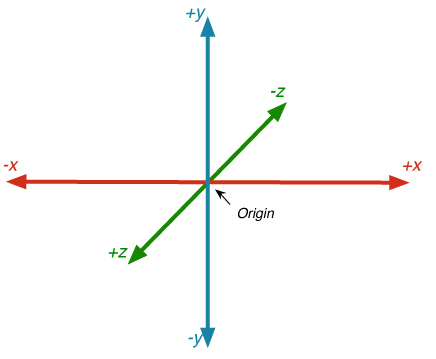
\includegraphics[width=0.5\textwidth]{Worldplane.png}
\caption{The axis of the world plane. A position in the world plane is given by (x,y,z) }
\end{figure}
\FloatBarrier

\begin{figure}[!h]
\centering
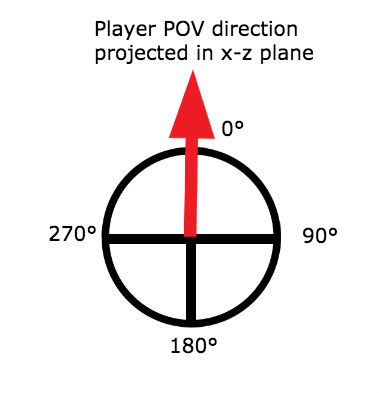
\includegraphics[width=0.5\textwidth]{POVZXPlane.jpg}
\caption{A visualization of the player POV projected on the x-z world plane. }
\end{figure}
\FloatBarrier

\subsection{Block Types}
The section deals with visually describing what each block type in BLOCK\_TYPES looks like.

\begin{figure}[!h]
  \begin{subfigure}[b]{0.25\textwidth}
    
\includegraphics[width=\textwidth]{GrassBlock.png}
    \caption{GRASS Block}
    \label{fig:f1}
  \end{subfigure}
  \hfill
  \begin{subfigure}[b]{0.4\textwidth}
    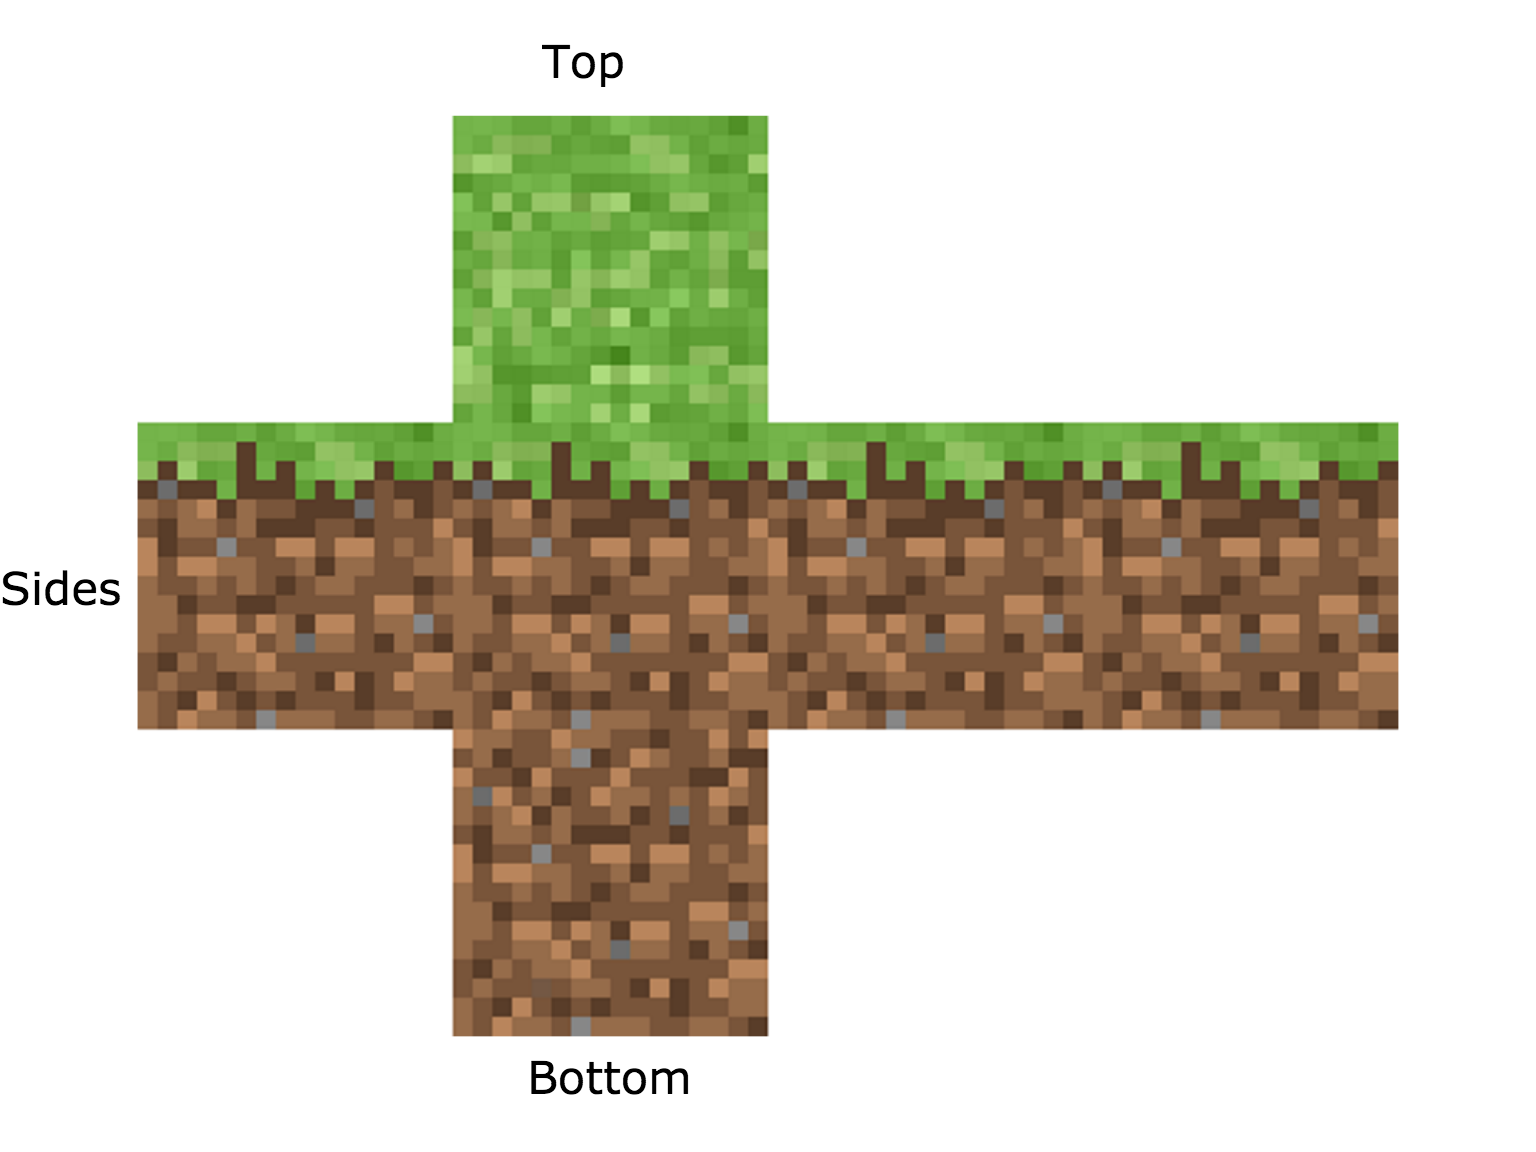
\includegraphics[width=\textwidth]{GrassTextures.png}
    \caption{GRASS block textures}
    \label{fig:f2}
  \end{subfigure}
  \caption{A visual of what the GRASS block type looks like}
\end{figure}

\begin{figure}[!tbp]
  \begin{subfigure}[b]{0.3\textwidth}
    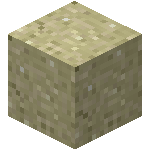
\includegraphics[width=\textwidth]{SandBlock.png}
    \caption{SAND Block}
    \label{fig:f1}
  \end{subfigure}
  \hfill
  \begin{subfigure}[b]{0.3\textwidth}
    
\includegraphics[width=\textwidth]{SandTexture.jpg}
    \caption{SAND block textures}
    \label{fig:f2}
  \end{subfigure}
  \caption{A visual of what the SAND block type looks like}
\end{figure}

\begin{figure}[!tbp]
  \begin{subfigure}[b]{0.3\textwidth}
    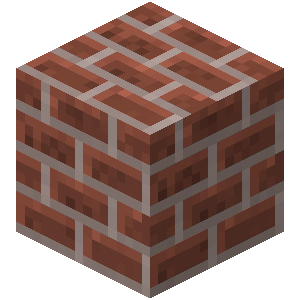
\includegraphics[width=\textwidth]{BrickBlock.png}
    \caption{BRICK Block}
    \label{fig:f1}
  \end{subfigure}
  \hfill
  \begin{subfigure}[b]{0.3\textwidth}
    
\includegraphics[width=\textwidth]{BrickTexture.png}
    \caption{BRICK block textures}
    \label{fig:f2}
  \end{subfigure}
  \caption{A visual of what the BRICK block type looks like}
\end{figure}

\newpage

\subsection{Symbolic Parameters}


The definition of the test cases will call for SYMBOLIC\_CONSTANTS.
Their values are defined in this section for easy maintenance.

\begin{tabular}{ |p{3cm}|p{3cm}|p{7cm}|  }
\hline
 Symbol & Value & Meaning\\
 \hline
 FRAME\_RATE & 60  & The frame rate the BlockBuilder will run at.\\
 \hline
 dt & 1/FRAME\_RATE seconds  & The time between each frame refresh.\\
 \hline
 SPEED & 5 units/s & The in game speed of the player \\
 \hline
 V & d = dt * SPEED  & The speed at which a player can move in any direction. \\
 \hline
 BLOCK\_SIZE & 1 unit  & The in-game side-length of a block.\\
 \hline
BLOCK\_TYPES & [GRASS, BRICK, SAND] & The types of blocks available to be placed by user. The block types depend on the skin they use defined in the Appendix.\\
 \hline
MAX\_BUILD\_D & 8 units  & The maximum distance the user must be to add or remove a block in a desired location.\\
 \hline
GRAVITY & 20 units/seconds  & A constant used to define the strength of the gravity.\\
 \hline
 UPTIME &99\%  & The uptime of the software.\\
 \hline
  AVAILTIME & 20 hours  & The time that the software should be available.\\
 \hline
   FLYING\_SPEED & 20 units/second  & The speed that the player can move in any direction when "flying mode" is entered.\\
 \hline
\end{tabular}

\subsection{Usability Survey Questions}

A results of a usability survey will be utilized to determine if BlockBuilder adequately meets the standards set by the original implementation. Example questions are the following:

\begin{itemize}
    \item On a scale of 1 to 5, how easy to use are the movement controls?
    \item Would you say the game is adequately smooth and lag-free?
    \item Are the building/destroying controls usable, in your opinion?
\end{itemize}

\end{document}